% ============================================================
%  GENERATED by make_a5.py — do not edit; edit the generator (or the master).
%  Space — A5 lesson booklet, 2027 workbook style.
%  The master is ../Space_Unit_Booklet_Yr7_8.tex (untouched).
%  Build: python3 make_a5.py && python3 fill_a5.py <jobname>
% ============================================================
\documentclass[11pt,a5paper,twoside]{article}

\usepackage{fontspec}
\setmainfont{Lato}[
  Path=../fonts/, Extension=.ttf, Ligatures=TeX,
  UprightFont=Lato-Regular, ItalicFont=Lato-Italic,
  BoldFont=Lato-Bold, BoldItalicFont=Lato-BoldItalic ]
% Headings in Outfit, the site's heading face. Bold is Outfit SemiBold, the
% weight the site uses; Outfit has no italic, so a slanted one stands in.
\newfontfamily\headingfont{Outfit}[
  Path=../fonts/, Extension=.ttf, Ligatures=TeX,
  UprightFont=Outfit-Regular, BoldFont=Outfit-SemiBold,
  ItalicFont=Outfit-Regular, ItalicFeatures={FakeSlant=0.18},
  BoldItalicFont=Outfit-SemiBold, BoldItalicFeatures={FakeSlant=0.18} ]

% A5, mirrored: the wider margin is on the inside, by the fold.
\usepackage[a5paper, inner=17mm, outer=13mm, top=19mm, bottom=17mm,
            headheight=14pt, headsep=4mm, footskip=8mm]{geometry}
\usepackage[protrusion=true,expansion=false]{microtype}
\usepackage{xcolor}
\usepackage{tikz}
\usetikzlibrary{arrows.meta, calc, patterns}
\usepackage{tcolorbox}
\tcbuselibrary{skins, breakable}
\usepackage{fancyhdr}
\usepackage{titlesec}
\usepackage{enumitem}
\usepackage{booktabs}
\usepackage{array}
\usepackage{longtable}
\usepackage{pdflscape}
\usepackage{amsmath}
\usepackage{needspace}
\usepackage{lastpage}
\usepackage{calc}
\usepackage{graphicx}
\usepackage{ragged2e}
\usepackage[hidelinks]{hyperref}

% ── Black and white inside ──────────────────────────────────────────────────
% The body still names the master's colours; inside an A5 booklet they all
% print as ink or grey, so map them here rather than editing the text.
\definecolor{Ink}{HTML}{111111}
\colorlet{Space}{Ink}\colorlet{SpaceMid}{Ink}\colorlet{Navy}{Ink}
\colorlet{DarkGrey}{black!72}\colorlet{Grey}{black!60}\colorlet{MidGrey}{black!35}
\colorlet{Line}{black!45}\colorlet{Paper}{white}\colorlet{LightGrey}{white}
\colorlet{Gold}{Ink}\colorlet{GoldDark}{Ink}\colorlet{Teal}{Ink}\colorlet{Coral}{Ink}
\colorlet{Violet}{Ink}\colorlet{Earth}{Ink}\colorlet{EarthDark}{Ink}
\color{Ink}

% ── Page style ──────────────────────────────────────────────────────────────
\pagestyle{fancy}
\fancyhf{}
\renewcommand{\headrulewidth}{0.4pt}
\fancyhead[LE]{\headingfont\footnotesize Space}
\fancyhead[RO]{\headingfont\footnotesize\leftmark}
\fancyfoot[LE,RO]{\headingfont\footnotesize\thepage}
\fancypagestyle{opener}{\fancyhf{}\renewcommand{\headrulewidth}{0pt}%
  \fancyfoot[LE,RO]{\headingfont\footnotesize\thepage}}
\raggedbottom
\setlength{\emergencystretch}{2em}
\setlength{\parindent}{0pt}
\setlength{\parskip}{4pt plus 1pt}
\setlist{itemsep=2pt, topsep=4pt, leftmargin=1.3em}

% ── Headings ────────────────────────────────────────────────────────────────
\titleformat{\subsection}{\headingfont\large\bfseries}{\thesubsection}{0.6em}{}
\titlespacing{\subsection}{0pt}{2pt}{6pt}
\titleformat{\subsubsection}{\headingfont\normalsize\bfseries}{}{0em}{}
\titlespacing{\subsubsection}{0pt}{8pt}{2pt}
% Every lesson part starts on a new page (Kodie's booklet rule).
\let\oldsubsection\subsection
\renewcommand{\subsection}{\clearpage\oldsubsection}

% ── Lesson opener band ──────────────────────────────────────────────────────
% \lessonopener{n}{title}{ink symbol}{running head}
\newcommand{\lessonopener}[4]{%
  \clearpage\thispagestyle{opener}%
  \refstepcounter{section}\markboth{#4}{#4}%
  \noindent\begin{minipage}[b]{\dimexpr\linewidth-34mm\relax}
    {\headingfont\bfseries\footnotesize\addfontfeatures{LetterSpace=14}SPACE \textbullet\ LESSON}\par\vspace{1mm}
    {\headingfont\bfseries\fontsize{46}{44}\selectfont #1}\par\vspace{2mm}
    {\headingfont\bfseries\fontsize{15}{18}\selectfont\RaggedRight #2\par}
  \end{minipage}\hfill
  \begin{minipage}[b]{31mm}\includegraphics[width=31mm]{#3}\end{minipage}\par
  \vspace{3mm}\noindent\rule{\linewidth}{1.6pt}\par\vspace{2mm}}

% Key vocabulary: a write-in table, one row per word, rows 1.5 cm tall,
% vertical rules between columns and down both sides (Kodie's table rule).
\newcommand{\vocabrow}[1]{\rule{0pt}{5mm}\textbf{#1}\rule[-10mm]{0pt}{0pt} & \\ \hline}
\newenvironment{keyvocab}{%
  \oldsubsection*{Key vocabulary}
  {\small Write what each word means as you meet it in this lesson.}\par\smallskip
  \renewcommand{\arraystretch}{1}%
  \begin{longtable}{|>{\RaggedRight}p{30mm}|p{\dimexpr\linewidth-30mm-4\tabcolsep-3\arrayrulewidth-1pt\relax}|}
  \hline \rule{0pt}{4.2mm}\headingfont\bfseries Word & \headingfont\bfseries What it means \\[1mm] \hline \endhead}
 {\end{longtable}}

% ── Box system: told apart by frame and icon, never by colour ───────────────
% Icons in the tab: I do ● · We do ●● · You do ●●● (the gradual release,
% read as dots), Key idea ◆, Above level ▲, Country ◎.
\newcommand{\icodots}[1]{\tikz[baseline=-0.6ex]{\foreach \i in {1,...,#1}{\fill[white] (\i*1.9mm,0) circle (0.7mm);}}}
\newcommand{\icokey}{\tikz[baseline=-0.6ex]{\fill[white] (0,0.9mm)--(0.9mm,0)--(0,-0.9mm)--(-0.9mm,0)--cycle;}}
\newcommand{\icoup}{\tikz[baseline=-0.6ex]{\fill[white] (-1mm,-0.8mm)--(1mm,-0.8mm)--(0,1mm)--cycle;}}
\newcommand{\icocountry}{\tikz[baseline=-0.6ex]{\draw[white,line width=0.5pt] (0,0) circle (1mm); \fill[white] (0,0) circle (0.45mm);}}
\tcbset{wbbase/.style={enhanced, colback=white, arc=1.2mm,
    left=3mm, right=3mm, top=4mm, bottom=2.5mm, before skip=10pt, after skip=8pt,
    attach boxed title to top left={xshift=3mm, yshift=-2.4mm},
    boxed title style={colback=Ink, colframe=Ink, arc=0.8mm, boxrule=0pt,
                       left=1.6mm, right=1.8mm, top=0.6mm, bottom=0.6mm},
    fonttitle=\headingfont\bfseries\footnotesize, coltitle=white}}
\newtcolorbox{idobox}[1]{wbbase, breakable, colframe=Ink, boxrule=1pt,
  title={\icodots{1}\ I do \textbullet\ #1}}
\newtcolorbox{wedobox}[1]{wbbase, breakable, frame hidden,
  borderline={1.1pt}{0pt}{Ink, dash pattern=on 4pt off 2.6pt},
  title={\icodots{2}\ We do \textbullet\ #1}}
\newtcolorbox{youdobox}[1][Check your understanding]{wbbase, breakable,
  colframe=Ink, boxrule=2.4pt, top=5mm,
  title={\icodots{3}\ You do \textbullet\ #1}}
\newtcolorbox{keybox}[1]{wbbase, breakable, colframe=Ink, boxrule=0.5pt,
  title={\icokey\ #1}}
\newtcolorbox{abovebox}[1][Above level \textbullet\ Year 8 extension]{wbbase, breakable, frame hidden,
  borderline={0.6pt}{0pt}{Ink}, borderline={0.6pt}{1.6pt}{Ink},
  title={\icoup\ #1}}
\newtcolorbox{countrybox}[1]{wbbase, breakable, frame hidden,
  borderline={1.4pt}{0pt}{Ink, line cap=round, dash pattern=on 0pt off 2.4pt},
  title={\icocountry\ #1}}

% ── Questions: number on its own line, text on the next, no marks ──────────
\newcounter{qnum}[section]
\renewcommand{\theqnum}{\thesection.\arabic{qnum}}
\newcommand{\question}[2]{\refstepcounter{qnum}\par\needspace{5\baselineskip}%
  \vspace{4pt}\noindent{\headingfont\bfseries Q\theqnum}\par\nobreak
  \noindent #2\par\nobreak\vspace{2pt}}
\newcommand{\vocab}[1]{\textbf{#1}}
\newcommand{\figcap}[1]{\begin{center}\small\itshape #1\end{center}}
\newcommand{\vc}[2]{{\small\itshape VC 2.0: #1 --- #2}\par}

% ── Writing space (from the Particle Model booklet, A5 sizes) ───────────────
% Every box logs its page to \jobname.abp; fill_a5.py measures the space left
% at the foot of each page and shares it out via \jobname.abx.
\newcounter{abox}
\newwrite\abpos \immediate\openout\abpos=\jobname.abp
\newcommand{\abset}[2]{\expandafter\gdef\csname abx@#1\endcsname{#2}}
\InputIfFileExists{\jobname.abx}{}{}
\def\abgrp{0}
\newcommand{\abnext}{\stepcounter{abox}%
  \edef\abcur{\ifcsname abx@\theabox\endcsname\csname abx@\theabox\endcsname\else 0pt\fi}}
\newcommand{\ablog}{\edef\abtmp{\noexpand\write\abpos{\theabox\space\abgrp\space\noexpand\thepage}}\abtmp}
\newcommand{\abh}[1]{\dimexpr#1+\abcur\relax}
% Plain box: mathematical working.
\newcommand{\workbox}[1]{\par\abnext
  \begin{tcolorbox}[enhanced, breakable=false, arc=1.2mm, colback=white, colframe=black!45,
    left=2mm, right=2mm, top=1mm, bottom=1mm, boxrule=0.8pt, height=\abh{#1}, before skip=3pt, after skip=6pt]
  \end{tcolorbox}\ablog}
% Dotted thirds: rows 9 mm, dotted / dotted / solid, ending on a dotted line;
% the number of rows comes from the box's final height. Dots stay dark.
\newlength\thirdrow \setlength\thirdrow{9mm}
\tikzset{thirdsolid/.style={draw=black!70, line width=0.5pt},
         thirddot/.style={draw=black!70, line width=0.6pt, dash pattern=on 0.9pt off 1.6pt}}
\newlength\lbH \newlength\lbO \newcount\lbN
\newcommand{\answerbox}[1]{\par\abnext
  \setlength\lbH{\dimexpr\abh{#1}-2pt\relax}%
  \lbN=\numexpr(\dimexpr\lbH-6mm-\thirdrow/2\relax)/\thirdrow\relax
  \ifnum\lbN<1 \lbN=1 \fi
  \setlength\lbO{\dimexpr(\lbH-\lbN\thirdrow)/2\relax}%
  \begin{tcolorbox}[enhanced, breakable=false, arc=1.2mm, colback=white, colframe=black!45,
    left=2mm, right=2mm, top=1mm, bottom=1mm, boxrule=0.8pt, height=\abh{#1}, before skip=3pt, after skip=6pt,
    underlay={\begin{tcbclipinterior}
      \foreach \i in {1,...,\the\lbN}{
        \draw[thirddot] ([xshift=3mm,yshift=-\lbO-(\i-1)*\thirdrow]interior.north west) -- ([xshift=-3mm,yshift=-\lbO-(\i-1)*\thirdrow]interior.north east);
        \draw[thirddot] ([xshift=3mm,yshift=-\lbO-(\i-1)*\thirdrow-\thirdrow/3]interior.north west) -- ([xshift=-3mm,yshift=-\lbO-(\i-1)*\thirdrow-\thirdrow/3]interior.north east);
        \draw[thirdsolid] ([xshift=3mm,yshift=-\lbO-(\i-1)*\thirdrow-2*\thirdrow/3]interior.north west) -- ([xshift=-3mm,yshift=-\lbO-(\i-1)*\thirdrow-2*\thirdrow/3]interior.north east);}
      \draw[thirddot] ([xshift=3mm,yshift=-\lbO-\lbN\thirdrow]interior.north west) -- ([xshift=-3mm,yshift=-\lbO-\lbN\thirdrow]interior.north east);
    \end{tcbclipinterior}}]
  \end{tcolorbox}\ablog}

% Ink fills for the labelling diagrams (no colour inside the booklet).
\tikzset{
  ink white/.style={fill=white},
  ink light/.style={preaction={fill=white}, pattern=north east lines},
  ink mid/.style={preaction={fill=white}, pattern=crosshatch},
  ink dots/.style={preaction={fill=white}, pattern=dots},
  ink rows/.style={preaction={fill=white}, pattern=horizontal lines},
  ink solid/.style={fill=Ink}}

% ── Padding to a multiple of 4 (copier booklet mode) ────────────────────────
\newcommand{\notespage}{\clearpage\markboth{Notes}{Notes}%
  \subsection*{Notes}\vspace{2mm}%
  \begin{tikzpicture}\foreach \y in {0,...,15}{\draw[black!35, line width=0.4pt] (0,-\y*9mm) -- (\linewidth,-\y*9mm);}\end{tikzpicture}}
\newcount\padleft
\newcommand{\padtofour}{\clearpage
  \pgfmathtruncatemacro\pagesused{\the\value{page}-1}%
  \pgfmathtruncatemacro\padn{mod(4-mod(\pagesused,4),4)}%
  \padleft=\padn\relax
  \loop\ifnum\padleft>0 \notespage\advance\padleft by -1 \repeat
  \clearpage}

\usetikzlibrary{shapes.geometric, positioning, decorations.pathreplacing, backgrounds}
\usepackage{colortbl}
\usepackage{tabularx}
\usepackage{multicol}
\usepackage{float}
\usepackage{bookmark}
\makeatletter\providecommand\Hy@PageAnchorSlide{}\makeatother
\colorlet{SpaceLight}{white}\colorlet{GoldLight}{white}\colorlet{CoralLight}{white}
\colorlet{TealLight}{white}\colorlet{VioletLight}{white}\colorlet{EarthLight}{white}
\colorlet{RowAlt}{white}\colorlet{TableHead}{Ink}
\arrayrulecolor{black!60}
\newcolumntype{L}[1]{>{\RaggedRight\arraybackslash}p{#1}}
\newcolumntype{C}[1]{>{\Centering\arraybackslash}p{#1}}
\newcommand{\thead}[1]{\headingfont\bfseries #1}
\newcommand{\talt}{}
\newcommand{\tmid}{\rowcolor{black!10}}
\newcommand{\markscount}[1]{}
\newenvironment{fillin}[1][2.6]{\begingroup\renewcommand{\arraystretch}{#1}}{\endgroup}
% A section that is all above level opens with this banner.
\newcommand{\extension}[1]{\begin{abovebox}[Above level \textbullet\ this whole lesson]#1\end{abovebox}}
% Moon phases and tides, from the master, in ink.
\colorlet{moonshadow}{black!80}\colorlet{moonlit}{white}\colorlet{moonink}{Ink}\colorlet{moonsoft}{black!60}
\newcommand{\moonR}{0.55}
\newcommand{\moonGap}{1.71}
\newcommand{\moonphase}[4]{%
	\begin{scope}[shift={(#1*\moonGap,0)}]
		\fill[moonshadow] (0,0) circle[radius=\moonR cm];
		\begin{scope}[xscale=#2]
			\fill[moonlit] (0,\moonR)
			arc[start angle=90,  end angle=-90, radius=\moonR cm]
			arc[start angle=-90, end angle=90,  x radius=#3*\moonR cm,
			y radius=\moonR cm] -- cycle;
		\end{scope}
		\draw[moonshadow, line width=0.4pt] (0,0) circle[radius=\moonR cm];
		\node[moonink, font=\scriptsize, align=center, anchor=north]
		at (0,-\moonR-0.14) {#4};
\end{scope}}
\colorlet{tideaccent}{black!80}\colorlet{tidewarm}{black!65}\colorlet{tidewarmsoft}{black!12}
\colorlet{tidecool}{black!10}\colorlet{tidefaint}{black!40}\colorlet{tidesoft}{black!55}
\newcommand{\tideunit}{0.021cm}
% A picture wider than the A5 text block is scaled down to fit it.
\newsavebox\fitb
\newenvironment{fitbox}{\begin{lrbox}{\fitb}}{\end{lrbox}%
  \ifdim\wd\fitb>\linewidth\resizebox{\linewidth}{!}{\usebox\fitb}\else\usebox\fitb\fi}
\newsavebox\tfitb
\newenvironment{tfitbox}{\begin{lrbox}{\tfitb}}{\end{lrbox}%
  \ifdim\wd\tfitb>\linewidth\resizebox{\linewidth}{!}{\usebox\tfitb}\else\usebox\tfitb\fi}

\begin{document}
\pdfbookmark[1]{Cover}{cover}
\thispagestyle{empty}
\begin{tikzpicture}[remember picture, overlay]
  \node at (current page.center) {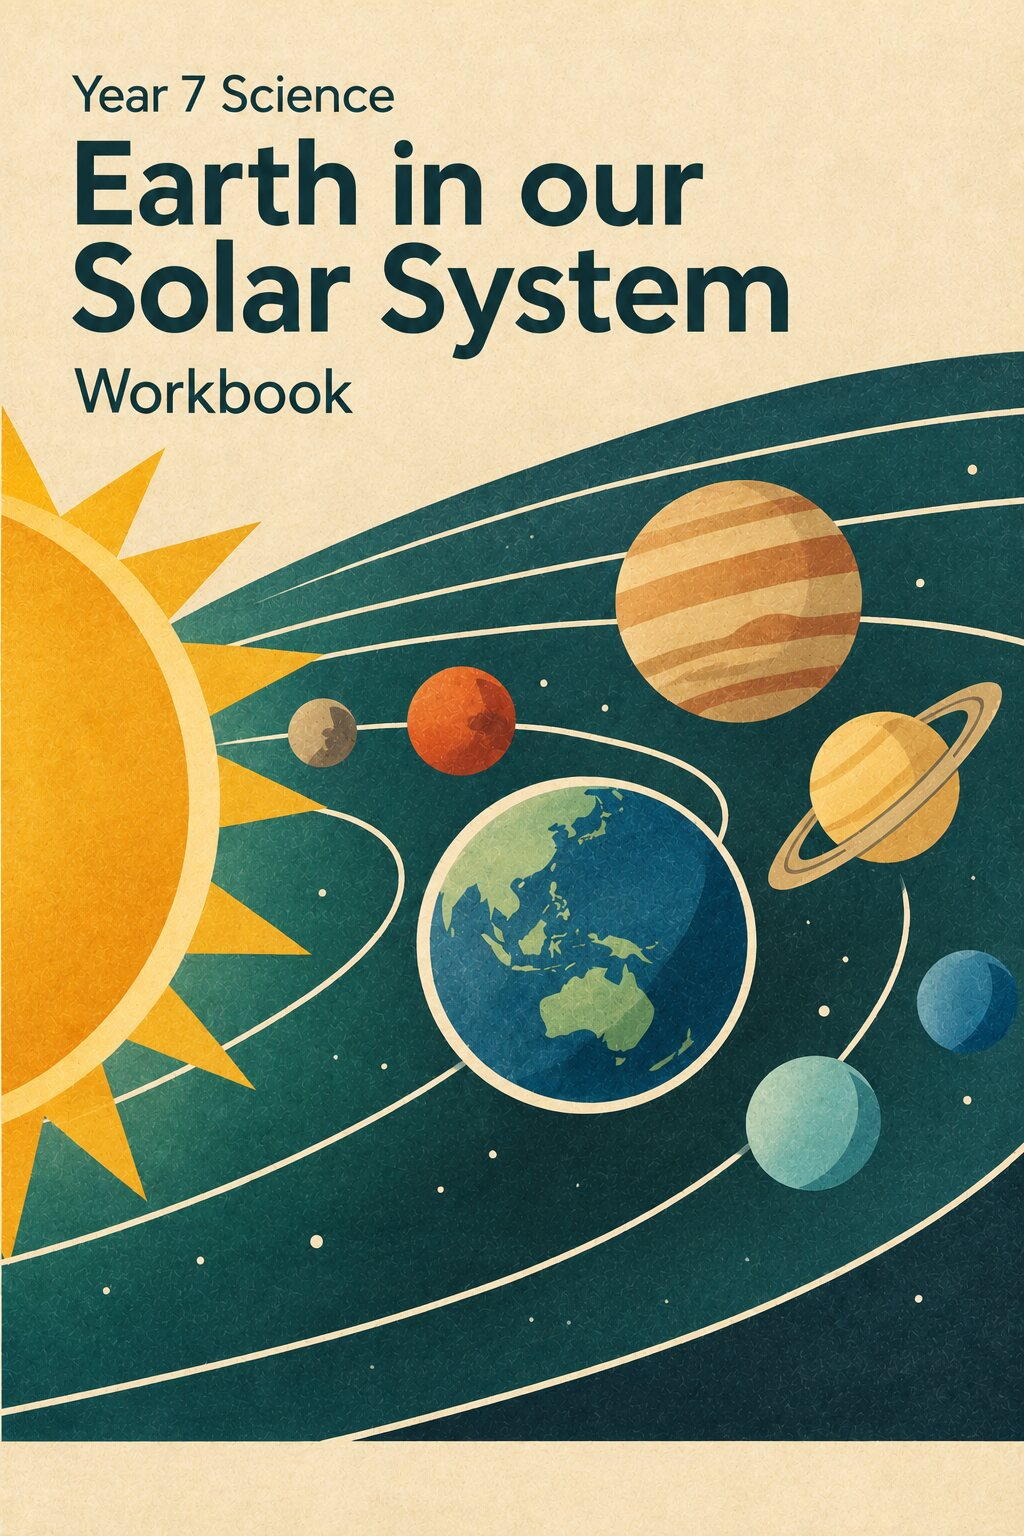
\includegraphics[width=\paperwidth, height=\paperheight, keepaspectratio=false, trim=0 40 0 40, clip]{../../../covers/earth-solar-system.jpg}};
  \node[anchor=north east, fill=white, draw=Ink, line width=0.6pt, rounded corners=1.5mm,
        inner xsep=2.4mm, inner ysep=2mm, text width=33mm, font=\headingfont\footnotesize]
    at ([xshift=-5mm, yshift=-4.5mm]current page.north east)
    {\textbf{Name}\par\vspace{4.2mm}\hrule\vspace{2.2mm}\textbf{Class}\par\vspace{4.2mm}\hrule};
  \node[anchor=south east, fill=white, draw=Ink, line width=0.6pt, rounded corners=1.2mm,
        inner xsep=2.6mm, inner ysep=2mm, font=\headingfont\bfseries, align=right]
    at ([xshift=-5mm, yshift=6mm]current page.south east)
    {Lesson Booklet\\[-1pt]{\normalfont\headingfont\scriptsize Lessons 1--7}};
\end{tikzpicture}
\mbox{}
\clearpage

\thispagestyle{plain}\markboth{Space}{Space}
{\headingfont\bfseries\Large Space}\par
{\headingfont Lesson Booklet \textbullet\ Lessons 1--7 \textbullet\ Year 7}\par\vspace{5mm}
\renewcommand{\arraystretch}{2.2}
\begin{tabular}{@{}l p{78mm}@{}}
\textbf{Name} & \hrulefill \\ \textbf{Class} & \hrulefill \\ \textbf{Teacher} & \hrulefill \\
\end{tabular}
\renewcommand{\arraystretch}{1}

\begin{countrybox}{Acknowledgement of Country}
This booklet was created on the unceded Country of the Wurundjeri-Woiwurrung people of the Kulin Nation. We acknowledge Elders past, present, and emerging. Aboriginal and Torres Strait Islander peoples have read, recorded and navigated by this sky for tens of thousands of years --- the oldest continuous astronomical tradition on Earth --- and that knowledge appears throughout this unit as living science, not history.
\end{countrybox}

\begin{keybox}{How this booklet works}
Section~N goes with Lesson~N. Each kind of box has its own frame and mark:\par\smallskip
\renewcommand{\arraystretch}{1.35}
\begin{tabular}{@{}p{24mm}l@{}}
\textbf{I do} {\scriptsize\textbullet} & Your teacher works it through --- you follow \\
\textbf{We do} {\scriptsize\textbullet\textbullet} & You try it with help, together \\
\textbf{You do} {\scriptsize\textbullet\textbullet\textbullet} & On your own: check your understanding \\
\textbf{Key idea} & The idea to remember \\
\textbf{Country} & First Nations perspectives (dotted frame) \\
\end{tabular}

\smallskip
One lesson book. The two labs are in the \textbf{Experiment Booklet}. Finished your lesson work and want to go further? Ask your teacher about \textbf{Advanced Space}.
\end{keybox}

\clearpage\markboth{Contents}{Contents}
\subsection*{Contents}
\renewcommand{\arraystretch}{1.35}
\begin{tabular}{|>{\Centering}p{11mm}|>{\RaggedRight}p{63mm}|>{\Centering}p{17mm}|}
  \hline\thead{Lesson} & \thead{Title} & \thead{Page} \\ \hline
  1 & \hyperlink{lesson.1.1}{Earth, Moon and Sun} & \hyperlink{lesson.1.1}{p.\ \pageref{sec:1}} \\ \hline
  2 & \hyperlink{lesson.2.1}{Day, Night and Seasons} \newline{\footnotesize\itshape + Experiment 1 --- The Angle of Sunlight (Experiment Booklet)} & \hyperlink{lesson.2.1}{p.\ \pageref{sec:2}} \\ \hline
  3 & \hyperlink{lesson.3.1}{Moon Phases and Tides} & \hyperlink{lesson.3.1}{p.\ \pageref{sec:3}} \\ \hline
  4 & \hyperlink{lesson.4.1}{Reading the Rocks} \textit{(optional)} & \hyperlink{lesson.4.1}{p.\ \pageref{sec:4}} \\ \hline
  5 & \hyperlink{lesson.5.1}{Our Solar System} \newline{\footnotesize\itshape + Experiment 2 --- Impact Craters (Experiment Booklet)} & \hyperlink{lesson.5.1}{p.\ \pageref{sec:5}} \\ \hline
  6 & \hyperlink{lesson.6.1}{Space Technology} & \hyperlink{lesson.6.1}{p.\ \pageref{sec:6}} \\ \hline
  7 & \hyperlink{lesson.7.1}{First Nations Astronomy} & \hyperlink{lesson.7.1}{p.\ \pageref{sec:7}} \\ \hline
  8 & \textit{The Search for Life} & Advanced Space \\ \hline
  9 & \textit{Gravity and Orbits} & Advanced Space \\ \hline
  10 & \textit{Stars, Galaxies and Starlight} & Advanced Space \\ \hline
  --- & \hyperlink{glossary}{Glossary} & \hyperlink{glossary}{\pageref{sec:glossary}} \\ \hline
\end{tabular}
\renewcommand{\arraystretch}{1}
\setcounter{section}{0}
\lessonopener{1}{Earth, Moon and Sun --- Scale and Structure}{../art/l1-ink.pdf}{1 \textbullet\ Earth, Moon and Sun}\label{sec:1}\pdfbookmark[1]{Lesson 1}{lesson.1}\hypertarget{lesson.1.1}{}
\vc{Science Understanding}{Physical sciences: Earth and space sciences; scale and relative size of Earth, Moon and Sun}

\begin{keyvocab}
  \vocabrow{Empty space}
  \vocabrow{Inner core}
  \vocabrow{Outer core}
  \vocabrow{Mantle}
  \vocabrow{Crust}
  \vocabrow{Satellite}
  \vocabrow{Regolith}
  \vocabrow{Tidal locking}
  \vocabrow{Highlands}
  \vocabrow{Maria}
  \vocabrow{Main sequence star}
  \vocabrow{Nuclear fusion}
\end{keyvocab}



\subsection{The scale of Earth, Moon and Sun}\label{sub:1.1}

The three most important objects in our immediate cosmic environment differ enormously in size. Understanding their relative sizes is foundational to everything else in this unit.

\begin{center}
\begin{tfitbox}\begin{tabular}{lrrr}
\toprule
\headingfont\textbf{Object} & \headingfont\textbf{Diameter (km)} & \headingfont\textbf{Mass (kg)} & \headingfont\textbf{Distance from Earth} \\
\midrule
Moon    & 3,474          & $7.34\times10^{22}$  & 384,400 km avg \\
Earth   & 12,742         & $5.97\times10^{24}$  & ---             \\
Sun     & 1,392,000      & $1.99\times10^{30}$  & 150,000,000 km (1 AU) \\
\bottomrule
\end{tabular}\end{tfitbox}
\end{center}

\begin{keybox}{Key concept: Scale}
If Earth were the size of a tennis ball (6.7 cm across), the Moon would be a marble (1.8 cm) about 1.9 m away, and the Sun would be a sphere 7.5 m across, placed 807 m down the road. The solar system is almost entirely \vocab{empty space}\label{voc:empty-space}.
\end{keybox}


\begin{youdobox}

\question{2}{Use the table to state the diameter of Earth and the diameter of the Sun.}
\answerbox{1.6cm}

\question{2}{Calculate how many times wider the Sun is than Earth. Show your working and give your answer to the nearest whole number.}
\workbox{1.6cm}

\question{2}{The Moon is 384,400 km from Earth. Calculate how many Earth diameters would fit into that gap.}
\workbox{1.6cm}

\question{2}{In the tennis-ball model, Earth is 6.7 cm across and the Sun sits 807 m down the road. Explain what this model shows that the table of diameters alone does not.}
\answerbox{1.6cm}

\end{youdobox}

\subsection{Structure of Earth}\label{sub:1.2}

Earth has four main layers:
\begin{itemize}
  \item \vocab{Inner core}\label{voc:inner-core} --- solid iron-nickel; radius \textasciitilde 1,200 km; temperature \textasciitilde 5,400°C
  \item \vocab{Outer core}\label{voc:outer-core} --- liquid iron-nickel; generates Earth's magnetic field (the dynamo effect)
  \item \vocab{Mantle}\label{voc:mantle} --- semi-solid rock; 2,900 km thick; convection currents drive plate tectonics
  \item \vocab{Crust}\label{voc:crust} --- thin, solid rock; 5--70 km thick; oceanic (denser, thinner) and continental (less dense, thicker)
\end{itemize}

\subsubsection{Diagram: Label the layers of Earth}
% Colours and band order mirror the slide-deck version of this diagram
% (deck1.html): the two outer layers in Space black, the two core layers
% in Gold. Leader lines run out to a common rail on the right so the
% labels sit in a single column and cannot collide.
\begin{center}
\begin{fitbox}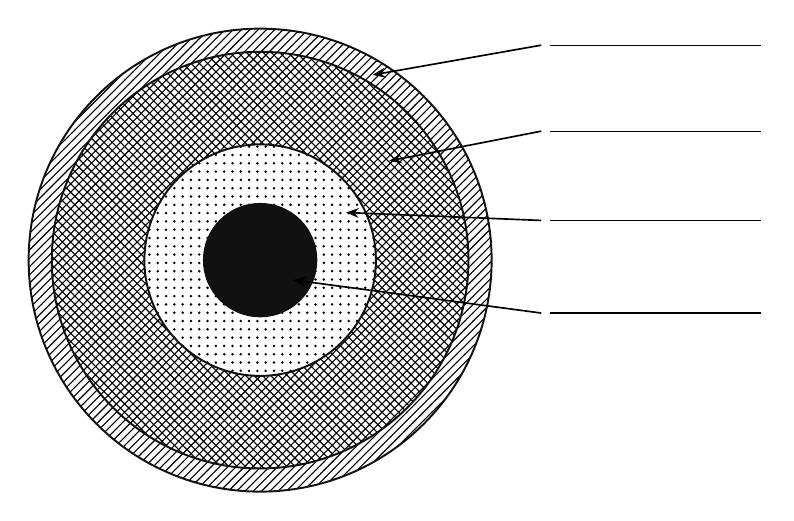
\begin{tikzpicture}[scale=0.84, every node/.style={transform shape},
    band/.style={draw=Ink, line width=0.7pt},
    lead/.style={draw=black, line width=0.6pt, -{Stealth[length=4.5pt,width=3.5pt]}},
    ansrule/.style={right, inner sep=2pt}
  ]
  \filldraw[band, ink light] (0,0) circle (3.5cm);
  \filldraw[band, ink mid] (0,0) circle (3.15cm);
  \filldraw[band, ink dots]  (0,0) circle (1.75cm);
  \filldraw[band, ink solid]  (0,0) circle (0.85cm);

  % arrowheads land inside the band being labelled
  \draw[lead] (4.25,3.25)  -- (1.70,2.8);
  \draw[lead] (4.25,1.95)  -- (1.95,1.5);
  \draw[lead] (4.25,0.60)  -- (1.30,0.72);
  \draw[lead] (4.25,-0.80) -- (0.50,-0.30);

  \node[ansrule] at (4.3,3.25)  {\rule{3.2cm}{0.5pt}};
  \node[ansrule] at (4.3,1.95)  {\rule{3.2cm}{0.5pt}};
  \node[ansrule] at (4.3,0.60)  {\rule{3.2cm}{0.5pt}};
  \node[ansrule] at (4.3,-0.80) {\rule{3.2cm}{0.5pt}};
\end{tikzpicture}\end{fitbox}

\vspace{0.6em}
{\small\textit{Word bank:}\quad Outer core \ \textbullet\ Crust \ \textbullet\ Inner core \ \textbullet\ Mantle}
\end{center}


\begin{youdobox}


\question{2}{Which layer generates Earth's magnetic field, and what is this process called?}
\answerbox{1.6cm}

\question{2}{The mantle is described as semi-solid rock. State its thickness and what its convection currents drive.}
\answerbox{1.6cm}

\question{2}{Compare oceanic and continental crust using two differences given in the booklet.}
\answerbox{1.6cm}

\end{youdobox}



\subsection{The Moon}\label{sub:1.3}

The Moon is Earth's only natural \vocab{satellite}\label{voc:satellite}. It produces no light of its own --- everything we see is reflected sunlight.

\begin{itemize}
  \item \textbf{Diameter}: 3,474 km --- about one quarter of Earth's
  \item \textbf{Distance}: 384,400 km from Earth on average; light crosses this in \textbf{1.28 seconds}
  \item \textbf{Orbital period}: 27.3 days --- and it \textit{rotates} in exactly the same time
  \item \textbf{Surface}: covered in \vocab{regolith}\label{voc:regolith}, a fine powdery rock produced by billions of years of meteorite impacts
  \item \textbf{No atmosphere} and no liquid water, so temperatures swing from $-173$\,°C at night to $+127$\,°C in daylight
\end{itemize}

\begin{keybox}{Why we only ever see one side}
The Moon's rotation period and orbital period are identical (27.3 days), so the same face is always turned towards Earth. This is called \vocab{tidal locking}\label{voc:tidal-locking}, and it is the normal outcome for a moon orbiting close to a much larger body. The hemisphere we never see from Earth is the \textbf{far side} --- not the ``dark side.'' It receives just as much sunlight as the near side.
\end{keybox}

Two kinds of terrain are visible with the naked eye. The number of craters on a surface tells you how old it is: the longer a surface has been there, the more impacts it has collected.

\begin{itemize}
  \item \vocab{Highlands}\label{voc:highlands} --- the bright, rugged regions. This is the Moon's \textbf{original crust}, so it is the oldest surface. It has been exposed to meteorite impacts for the whole history of the Moon, which is why it is so heavily cratered
  \item \vocab{Maria}\label{voc:maria} (singular \textit{mare}, Latin for ``sea'') --- the dark, flat plains. Later, huge impacts punched basins into the crust, and lava welled up and flooded them. When that lava cooled it created a \textbf{new, smooth surface}, wiping out the craters that were there before. Because this happened after the highlands formed, the maria have had less time to collect impacts --- so they are only lightly cratered
\end{itemize}


\begin{youdobox}

\question{3}{Explain why we always see the same face of the Moon from Earth.}
\answerbox{1.6cm}

\question{2}{Describe the difference between the maria and the highlands, and state which is older.}
\answerbox{1.6cm}

\question{2}{The Moon has no atmosphere. Explain how this causes its extreme temperature range.}
\answerbox{1.6cm}

\end{youdobox}



\subsection{Structure of the Sun}\label{sub:1.4}

The Sun is a \vocab{main sequence star}\label{voc:main-sequence-star} --- it converts hydrogen into helium through \vocab{nuclear fusion}\label{voc:nuclear-fusion} in its core.

\begin{itemize}
  \item \textbf{Core}: where fusion occurs; temperature \textasciitilde 15 million°C
  \item \textbf{Radiative zone}: energy moves outward as photons (takes \textasciitilde 100,000 years to cross)
  \item \textbf{Convective zone}: energy carried by convecting plasma
  \item \textbf{Photosphere}: the visible surface (\textasciitilde 5,778 K); where sunspots form
  \item \textbf{Chromosphere and Corona}: outer atmosphere; much hotter than photosphere (corona: 1--3 million K)
\end{itemize}

\subsubsection{Diagram: Label the layers of the Sun}
% Same construction as the Earth diagram in 1.2.1 — concentric bands,
% white separators, leader lines out to a common rail on the right.
% Warm palette here rather than Space blue: gold ramp for the interior,
% Coral for the fusion core and the chromosphere.
\begin{center}
\begin{fitbox}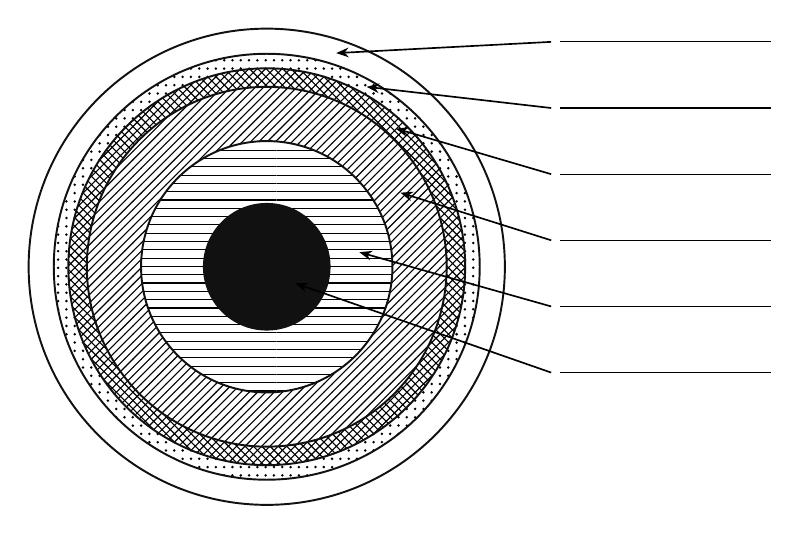
\begin{tikzpicture}[scale=0.84, every node/.style={transform shape},
    band/.style={draw=Ink, line width=0.7pt},
    lead/.style={draw=black, line width=0.6pt, -{Stealth[length=4.5pt,width=3.5pt]}},
    ansrule/.style={right, inner sep=2pt}
  ]
  \filldraw[band, ink white]     (0,0) circle (3.60cm);
  \filldraw[band, ink dots]    (0,0) circle (3.22cm);
  \filldraw[band, ink mid] (0,0) circle (3.00cm);
  \filldraw[band, ink light]     (0,0) circle (2.72cm);
  \filldraw[band, ink rows]     (0,0) circle (1.90cm);
  \filldraw[band, ink solid]    (0,0) circle (0.95cm);

  \draw[lead] (4.30,3.40)  -- (1.05,3.23);
  \draw[lead] (4.30,2.40)  -- (1.51,2.72);
  \draw[lead] (4.30,1.40)  -- (1.95,2.09);
  \draw[lead] (4.30,0.40)  -- (2.02,1.12);
  \draw[lead] (4.30,-0.60) -- (1.40,0.22);
  \draw[lead] (4.30,-1.60) -- (0.43,-0.25);

  \node[ansrule] at (4.35,3.40)  {\rule{3.2cm}{0.5pt}};
  \node[ansrule] at (4.35,2.40)  {\rule{3.2cm}{0.5pt}};
  \node[ansrule] at (4.35,1.40)  {\rule{3.2cm}{0.5pt}};
  \node[ansrule] at (4.35,0.40)  {\rule{3.2cm}{0.5pt}};
  \node[ansrule] at (4.35,-0.60) {\rule{3.2cm}{0.5pt}};
  \node[ansrule] at (4.35,-1.60) {\rule{3.2cm}{0.5pt}};
\end{tikzpicture}\end{fitbox}

\vspace{0.6em}
{\small\textit{Word bank:}\quad Convective zone \ \textbullet\ Corona \ \textbullet\ Core \ \textbullet\ Photosphere \ \textbullet\ Chromosphere \ \textbullet\ Radiative zone}
\end{center}

\begin{idobox}{Worked example: Light travel time from the Sun}
\textit{The Sun is 150,000,000 km from Earth. Light travels at 300,000 km/s. How long does sunlight take to reach us?}

\medskip
$\text{Time} = \dfrac{\text{Distance}}{\text{Speed}} = \dfrac{150{,}000{,}000 \text{ km}}{300{,}000 \text{ km/s}} = 500 \text{ s} = 8 \text{ min } 20 \text{ s}$

\medskip
\textbf{Answer}: Sunlight takes 8 minutes and 20 seconds to reach Earth. This means the Sun we see right now is actually how it looked 8 minutes ago.
\end{idobox}

\begin{wedobox}{Your turn}
A flash of light leaves the Moon. How long before we see it? (Moon is 384,400 km away; speed of light = 300,000 km/s)

\workbox{4cm}
\end{wedobox}


\begin{youdobox}

\question{2}{Define nuclear fusion as it occurs in the Sun.}
\answerbox{1.6cm}

\question{2}{State the temperature of the Sun's core and of its photosphere.}
\answerbox{1.6cm}

\question{3}{Jupiter is 5.20 AU from the Sun. Sunlight reaches Earth (1 AU) in 500 seconds. Calculate how long sunlight takes to reach Jupiter, in minutes and seconds.}
\workbox{1.6cm}

\end{youdobox}



\setcounter{section}{1}
\lessonopener{2}{Day, Night and Seasons}{../art/l2-ink.pdf}{2 \textbullet\ Day, Night and Seasons}\label{sec:2}\pdfbookmark[1]{Lesson 2}{lesson.2}\hypertarget{lesson.2.1}{}
\vc{Science Understanding}{Earth and space sciences: Earth's rotation and revolution; axial tilt and seasons}

\begin{keyvocab}
  \vocabrow{Rotates}
  \vocabrow{West to east}
  \vocabrow{Revolves}
  \vocabrow{Axial tilt}
\end{keyvocab}


\subsection{Why we have day and night}\label{sub:2.1}

Earth \vocab{rotates}\label{voc:rotates} (spins on its axis) once every \textbf{24 hours}. The side facing the Sun experiences day; the opposite side experiences night.

\begin{itemize}
  \item Earth rotates \vocab{west to east}\label{voc:west-to-east} (anticlockwise when viewed from above the North Pole)
  \item This is why the Sun appears to rise in the east and set in the west
  \item Earth also \vocab{revolves}\label{voc:revolves} (orbits) around the Sun once every 365.25 days --- one year
\end{itemize}

\begin{wedobox}{Draw it: day and night}
Copy the simple diagram showing \textbf{Earth and the Sun}. On your diagram:
\begin{itemize}
  \item shade the half of Earth where it is \textbf{night}, and label the half where it is \textbf{day}
  \item draw an arrow showing the direction of the Sun's light
  \item add a curved arrow showing which way Earth \textbf{rotates}
\end{itemize}

\workbox{5cm}
\end{wedobox}

\begin{youdobox}

\question{2}{State how long Earth takes to rotate once on its axis, and how long it takes to revolve once around the Sun.}
\answerbox{1.6cm}

\question{2}{Explain why the Sun appears to rise in the east and set in the west.}
\answerbox{1.6cm}

\end{youdobox}

\subsection{Why we have seasons}\label{sub:2.2}

Seasons are caused by Earth's \vocab{axial tilt}\label{voc:axial-tilt} of 23.5°, not by distance from the Sun. (Earth is actually closest to the Sun in January --- Australian summer.)

% Axial tilt reference diagram. Mirrors the version on the deck 2 theory
% slide: the angle is measured between the rotation axis and the
% perpendicular to the orbital plane. Note the equator is drawn
% perpendicular to the AXIS (-23.5°/156.5°), not to the vertical.
\begin{center}
\begin{fitbox}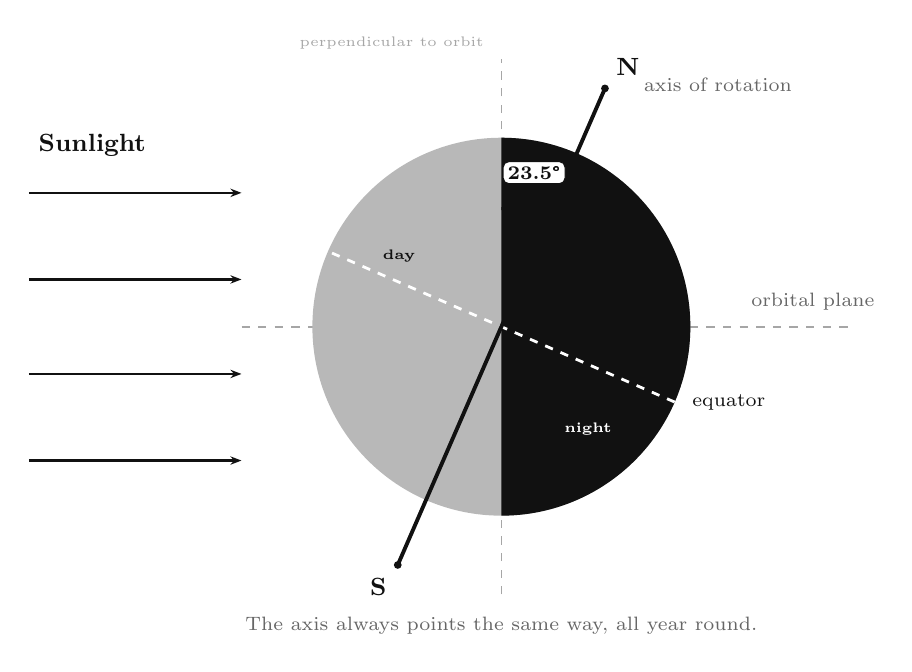
\begin{tikzpicture}[x=1cm,y=1cm]
  \def\R{2.4}
  \draw[MidGrey, dashed, line width=0.7pt] (-3.3,0) -- (4.5,0);
  \node[Grey, font=\scriptsize, anchor=west] at (3.05,0.32) {orbital plane};
  \foreach \y in {1.7,0.6,-0.6,-1.7}{
    \draw[Gold, line width=0.9pt, -{Stealth[length=4pt]}] (-6.0,\y) -- (-3.3,\y);
  }
  \node[Gold, font=\bfseries\small, anchor=west] at (-6.0,2.3) {Sunlight};

  \draw[MidGrey, dashed, line width=0.6pt] (0,-3.4) -- (0,3.4);
  \node[MidGrey, font=\tiny, anchor=south east] at (-0.1,3.4) {perpendicular to orbit};

  \fill[Space!30] (0,0) circle (\R);
  \fill[Navy] (0,\R) arc (90:-90:\R) -- cycle;
  \node[Ink, font=\bfseries\tiny] at (-1.3,0.9) {day};
  \node[white, font=\bfseries\tiny] at (1.1,-1.3) {night};

  \draw[white, dashed, line width=1pt] (-23.5:\R) -- (156.5:\R);
  \node[Ink, font=\scriptsize, anchor=west] at (-23.5:\R) {\hspace{1mm}equator};

  \draw[Ink, line width=1.4pt] (66.5:3.3) -- (246.5:3.3);
  \fill[Ink] (66.5:3.3) circle (1.4pt);  \fill[Ink] (246.5:3.3) circle (1.4pt);
  \node[Ink, font=\bfseries\small, anchor=south west] at (66.5:3.35) {N};
  \node[Ink, font=\bfseries\small, anchor=north east] at (246.5:3.35) {S};
  \node[Grey, font=\scriptsize, anchor=west] at (66.5:3.35) {\hspace{3.5mm}axis of rotation};

  \draw[Gold, line width=1.1pt] (90:1.5) arc (90:66.5:1.5);
  \node[fill=GoldLight, draw=Gold, rounded corners=2pt, inner sep=1.6pt,
        text=GoldDark, font=\bfseries\scriptsize] at (78:2.0) {23.5\textdegree};

  \node[Grey, font=\scriptsize] at (0,-3.8) {The axis always points the same way, all year round.};
\end{tikzpicture}\end{fitbox}
\end{center}

\begin{keybox}{Why tilt causes seasons}
When the Southern Hemisphere tilts toward the Sun (December):
\begin{itemize}
  \item The Sun is higher in the sky --- its rays hit at a more direct angle (more energy per m$^2$)
  \item Days are longer --- more hours of sunlight
  \item The combination produces \textbf{summer} in Australia
\end{itemize}
When the Southern Hemisphere tilts away (June): rays hit at a shallower angle, days are shorter --- \textbf{winter}.
\end{keybox}


\begin{youdobox}

\question{1}{State the size of Earth's axial tilt.}
\answerbox{1.6cm}

\question{2}{State two effects of the Southern Hemisphere being tilted toward the Sun in December.}
\answerbox{1.6cm}

\question{3}{Earth is actually closest to the Sun in January. Explain why this is \textit{not} the cause of Australian summer.}
\answerbox{1.6cm}

\end{youdobox}


\subsection{Solstices and equinoxes}\label{sub:2.3}

\begin{center}
\begin{tfitbox}\begin{tabular}{@{}L{2.46cm}L{2.36cm}L{5.71cm}@{}}
\toprule
\textbf{Event} & \textbf{Date (approx.)} & \textbf{What happens} \\
\midrule
December solstice & 21--22 December & Southern Hemisphere longest day; summer solstice for Australia \\
June solstice     & 21--22 June     & Southern Hemisphere shortest day; winter solstice for Australia \\
March equinox     & 20--21 March    & Equal day/night worldwide; autumn begins in Australia \\
September equinox & 22--23 September& Equal day/night worldwide; spring begins in Australia \\
\bottomrule
\end{tabular}\end{tfitbox}
\end{center}



\begin{wedobox}{Your turn}
Apply your knowledge — attempt all three, then we’ll reveal answers:

\textbf{Q1:} It is March 21 (equinox) in Melbourne. Is it day or night at the North Pole right now?
\answerbox{5.0cm}
\textbf{Q2:} A student in Brazil says “We’re having summer right now.” What month is it most likely to be?
\answerbox{5.0cm}
\textbf{Q3:} Earth is actually slightly closer to the Sun in January than in July. Why is it still winter in Scandinavia in January?
\answerbox{5.0cm}
\end{wedobox}


\begin{youdobox}

\question{2}{Using the table, state the date of the Australian summer solstice and what happens on that day.}
\answerbox{1.6cm}

\question{2}{State what is equal at an equinox, and name the Australian season that begins at the March equinox.}
\answerbox{1.6cm}

\end{youdobox}
\setcounter{section}{2}
\lessonopener{3}{The Moon --- Phases and Tides}{../art/l3-ink.pdf}{3 \textbullet\ Moon Phases and Tides}\label{sec:3}\pdfbookmark[1]{Lesson 3}{lesson.3}\hypertarget{lesson.3.1}{}
\vc{Science Understanding}{Earth and space sciences: Moon phases and tidal patterns; gravitational effects}

\begin{keyvocab}
  \vocabrow{Reflects sunlight}
  \vocabrow{Phases}
  \vocabrow{Lunar eclipse}
  \vocabrow{Tidal bulge}
  \vocabrow{Spring tides}
  \vocabrow{Neap tides}
\end{keyvocab}



\subsection{Why the Moon appears to change shape}\label{sub:3.1}

The Moon does not produce light --- it \vocab{reflects sunlight}\label{voc:reflects-sunlight}. At all times, the half facing the Sun is lit. As the Moon orbits Earth, we see different fractions of the lit half from Earth --- these are the \vocab{phases}\label{voc:phases}. One orbit takes \textbf{27.3 days}, but a full cycle of phases takes \textbf{29.5 days}: Earth moves along its own orbit at the same time, so the Moon needs about two more days to line up with the Sun again.
\subsubsection{The eight phases (in order), as seen from Melbourne}
\begin{center}
	\begin{fitbox}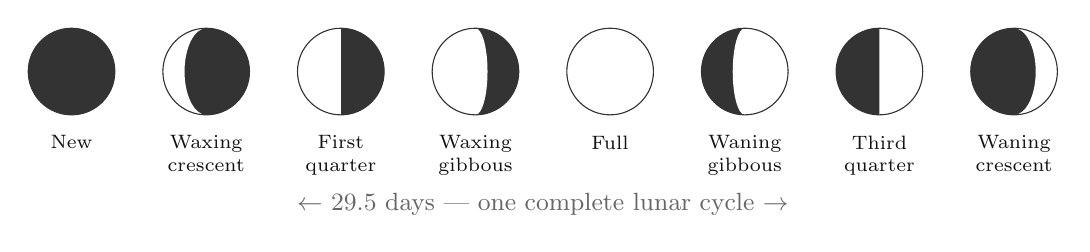
\begin{tikzpicture}[x=1cm, y=1cm]
	% As seen from Melbourne: waxing is lit on the LEFT (-1).
	\moonphase{0}{-1}{ 1.000}{New}
	\moonphase{1}{-1}{ 0.500}{Waxing\\crescent}
	\moonphase{2}{-1}{ 0.000}{First\\quarter}
	\moonphase{3}{-1}{-0.278}{Waxing\\gibbous}
	\moonphase{4}{ 1}{-1.000}{Full}
	\moonphase{5}{ 1}{-0.278}{Waning\\gibbous}
	\moonphase{6}{ 1}{ 0.000}{Third\\quarter}
	\moonphase{7}{ 1}{ 0.500}{Waning\\crescent}
	\node[moonsoft, font=\small] at (3.5*\moonGap,-1.68)
	{$\leftarrow$ 29.5 days --- one complete lunar cycle $\rightarrow$};
\end{tikzpicture}\end{fitbox}
\end{center}

\begin{keybox}{Which side is lit depends on where you are standing}
From Australia a \textbf{waxing} Moon is lit on the \textbf{left}, and a \textbf{waning} Moon is lit on the \textbf{right} --- exactly the opposite of most textbook and internet diagrams, which are drawn for the Northern Hemisphere. Nothing about the Moon is different; an observer in Melbourne is simply standing ``upside down'' relative to one in London, so the same lit half is seen rotated by 180$^\circ$. The row above is drawn as you would actually see it from the school yard.
\end{keybox}

\begin{keybox}{Common misconception}
Earth's shadow does \textbf{NOT} cause phases. A \vocab{lunar eclipse}\label{voc:lunar-eclipse} (Earth's shadow on the Moon) is a separate, less frequent event. Phases are caused by our changing view of the Moon's lit half.
\end{keybox}


\begin{youdobox}

\question{1}{State how long the Moon takes to complete one full cycle of phases.}
\answerbox{1.6cm}

\question{3}{Explain why the Moon appears to change shape over a month.}
\answerbox{1.6cm}

\question{2}{A student writes: ``The phases of the Moon are caused by Earth's shadow falling on it.'' Correct this statement.}
\answerbox{1.6cm}

\end{youdobox}

\subsection{Tides}\label{sub:3.2}

The Moon's gravity pulls on Earth's oceans. This creates a \vocab{tidal bulge}\label{voc:tidal-bulge} on the Moon-facing side, and a second bulge on the opposite side.

\begin{itemize}
  \item \vocab{Spring tides}\label{voc:spring-tides}: Sun, Earth, and Moon are aligned (new or full Moon). Gravitational pulls add together --- very large tidal range
  \item \vocab{Neap tides}\label{voc:neap-tides}: Moon at right angles to the Sun--Earth line (quarter phases). Pulls partially cancel --- moderate tidal range
  \item ``Spring'' refers to the Old English word for ``to leap,'' not the season
\end{itemize}
\begin{center}
	\begin{fitbox}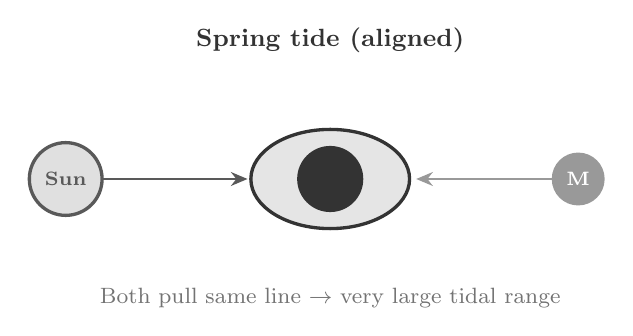
\begin{tikzpicture}[x=\tideunit, y=-\tideunit,   % y flipped: SVG coords
	every node/.style={inner sep=0pt},
	arr/.style={line width=1pt,
		-{Stealth[length=6pt, width=5pt]}}]
	
	\node[font=\bfseries\small, text=tideaccent] at (190,16)
	{Spring tide (aligned)};
	
	% Sun
	\filldraw[fill=tidewarmsoft, draw=tidewarm, line width=1.2pt]
	(30,100) circle[radius=22];
	\node[font=\bfseries\scriptsize, text=tidewarm] at (30,100) {Sun};
	
	% Earth: tidal-bulge envelope, then the solid planet
	\filldraw[fill=tidecool, draw=tideaccent, line width=1.2pt]
	(190,100) ellipse[x radius=48, y radius=30];
	\fill[tideaccent] (190,100) circle[radius=20];
	
	% Moon
	\fill[tidefaint] (340,100) circle[radius=16];
	\node[font=\bfseries\scriptsize, text=white] at (340,100) {M};
	
	% Pull arrows
	\draw[arr, tidewarm]  (52,100)  -- (140,100);
	\draw[arr, tidefaint] (324,100) -- (242,100);
	
	\node[font=\footnotesize, text=tidesoft] at (190,172)
	{Both pull same line $\rightarrow$ very large tidal range};
\end{tikzpicture}\end{fitbox}
\end{center}

% Working space for the "You do" on lesson 3, slide 7. Unnumbered, like the
% other "Your turn" blocks, so it does not disturb the \question sequence.
% Deliberately about tides only: eclipses are Year 8 extension material in
% this unit, so a You-do on them would sit above the level.
\begin{wedobox}{Your turn: spring and neap tides}
There is a \textbf{full Moon} on 5 March.

\medskip
\textbf{(a)} What kind of tides would you expect that week --- spring or neap? Explain your answer using the positions of the Sun, Earth and Moon.
\answerbox{5.0cm}

\medskip
\textbf{(b)} Roughly how many days later would you next expect \textbf{neap} tides, and what phase will the Moon be then?
\answerbox{5.0cm}

\medskip
\textbf{(c)} Why does one place on Earth get \textbf{two} high tides in a day, rather than just one?
\answerbox{5.0cm}
\end{wedobox}




\begin{youdobox}

\question{1}{State what causes the tidal bulge on the side of Earth facing the Moon.}
\answerbox{1.6cm}

\question{3}{Explain the difference between spring tides and neap tides, including when each occurs.}
\answerbox{1.6cm}

\end{youdobox}


\setcounter{section}{3}
\lessonopener{4}{Reading the Rocks --- Tides in Stone and the Acraman Impact}{../art/l4-ink.pdf}{4 \textbullet\ Reading the Rocks}\label{sec:4}\pdfbookmark[1]{Lesson 4}{lesson.4}\hypertarget{lesson.4.1}{}
\vc{Science as a Human Endeavour}{Science knowledge is used to inform decisions and is developed through the work of individual scientists; Earth and space sciences: predictable phenomena}

\begin{keyvocab}
  \vocabrow{Tidal rhythmite}
  \vocabrow{Lamina}
  \vocabrow{Elatina Formation}
  \vocabrow{Tidal braking}
  \vocabrow{Planar deformation features}
\end{keyvocab}



Everything so far in this unit has been observed by looking \emph{up}. This
section does the opposite. Two sets of South Australian rocks, both studied by
\textbf{Professor George Williams} at the University of Adelaide, record events
that happened in space --- one a rhythm repeated for sixty years, the other a
single morning that changed the planet. \textbf{We hold samples of both}, so
this section is written to be worked through with the specimens in front of
you.

\subsection{Tides written in stone}\label{sub:4.1}

\begin{wedobox}{Entry task: what could you count in a rock?}
The photograph on the poster shows a slab of rock made of hundreds of thin,
regular layers, each one a fraction of a millimetre thick. Before you read on:
what natural process could lay down a layer of sediment that regularly, and
what would counting the layers tell you?
\answerbox{5.0cm}
\end{wedobox}

A \vocab{tidal rhythmite}\label{voc:tidal-rhythmite} is a sedimentary rock made of finely layered silt and
sand laid down by tidal currents. Each incoming tide carries sediment into a
tidal inlet and drops it as a thin layer, called a \vocab{lamina}\label{voc:lamina}. A stronger
tide carries more sediment and leaves a thicker lamina.

That makes a rhythmite a \textbf{recording} of the tides, in the same way a
tree's rings record its years:

\begin{itemize}
  \item one \textbf{lamina} = one tidal cycle (roughly one lunar day)
  \item laminae get thicker and thinner on a fortnightly cycle --- the
        \textbf{spring} and \textbf{neap} tides you met in Section 2
  \item counting laminae between one neap and the next gives the number of days
        in a lunar month, \emph{at the time the rock formed}
\end{itemize}

The \vocab{Elatina Formation}\label{voc:elatina-formation} in the Flinders Ranges is a rhythmite
\textbf{635 million years} old. Williams analysed a 10 m drill core holding a
continuous 60-year record and counted:

\begin{center}
\begin{tfitbox}\begin{tabular}{lrr}
\toprule
\headingfont\textbf{Measurement} & \headingfont\textbf{635 Ma} & \headingfont\textbf{Today} \\
\midrule
Solar days per lunar month & $30.5 \pm 0.5$ & 29.53 \\
Lunar months per year      & $13.1 \pm 0.1$ & 12.37 \\
Solar days per year        & $400 \pm 7$    & 365.24 \\
Length of a solar day (hours) & $21.9 \pm 0.4$ & 24.00 \\
\bottomrule
\end{tabular}\end{tfitbox}
\end{center}

\begin{keybox}{The year did not change --- the day did}
$400 \times 21.9 = 8760$ hours. $365.24 \times 24.00 = 8766$ hours. The two
agree to better than 0.1\%. Earth took just as long to go round the Sun 635
million years ago as it does now --- it simply \textbf{spun faster}, so more
days fitted into the same year.
\end{keybox}

\subsubsection{Why Earth is slowing down}

The Moon raises a tidal bulge in Earth's oceans. Earth rotates faster than the
Moon orbits, so friction drags that bulge slightly \emph{ahead} of the Moon.
The bulge pulls the Moon forward, and the Moon pulls back on Earth.

\begin{itemize}
  \item Earth loses rotational energy --- \textbf{the day gets longer}
  \item the Moon gains orbital energy --- \textbf{the Moon moves further away}
\end{itemize}

This is called \vocab{tidal braking}\label{voc:tidal-braking}. Laser reflectors left on the Moon by
Apollo astronauts let us measure the recession directly today:
\textbf{3.8 cm per year}.

The rhythmites let us check that figure against the deep past, and the answer
is interesting: averaged over the last 635 million years the Moon receded at
only about \textbf{2 cm per year} --- barely half today's rate. The rate is not
a constant. It depends on the shape of the ocean basins, which changes as the
continents drift.

\begin{keybox}{Why this matters for where the Moon came from}
Any explanation of the Moon's origin has to produce an orbit that behaves the
way the rocks say it behaved. Assume today's recession rate has always applied,
wind the clock back, and you get an Earth--Moon history that does not fit a
4.5-billion-year-old Moon. The rhythmites are one of very few
\textbf{direct measurements} of the ancient Earth--Moon system, so they are
used to test the models rather than trust them. The currently accepted
explanation --- a Mars-sized body striking the young Earth and throwing debris
into orbit --- rests mostly on other evidence (the Moon's tiny iron core, and
lunar rock chemistry that matches Earth's mantle almost exactly).
\end{keybox}

\begin{youdobox}

\question{1}{State what one lamina in a tidal rhythmite represents.}
\answerbox{1.6cm}

\question{2}{Explain why laminae in a rhythmite vary in thickness on a fortnightly cycle.}
\answerbox{1.6cm}

\question{2}{Using the table, state how many days there were in a year 635 million years ago, and how long a day was.}
\answerbox{1.6cm}

\question{3}{Show that a 400-day year of 21.9-hour days is about the same length as our year of 365.24 days. Explain what this tells you about Earth's orbit compared with Earth's spin.}
\answerbox{1.6cm}

\question{3}{Describe how tidal braking makes Earth's day longer and pushes the Moon further away. Refer to the tidal bulge in your answer.}
\answerbox{1.6cm}

\question{2}{The Moon currently recedes at 3.8 cm per year, but the average over the last 635 million years was about 2 cm per year. State what this shows about the recession rate, and give one reason it changes.}
\answerbox{1.6cm}

\end{youdobox}

\subsection{The Acraman impact}\label{sub:4.2}

\begin{wedobox}{Entry task: what would be left behind?}
An asteroid 5 km across hits South Australia. 580 million years of erosion
follow. List three things you would look for today as evidence that it
happened.
\answerbox{5.0cm}
\end{wedobox}

About \textbf{580 million years ago} an asteroid roughly \textbf{5 km across},
travelling at \textbf{25 km per second}, struck the Gawler Range Volcanics in
what is now the Gawler Ranges of South Australia.

\begin{center}
\begin{tfitbox}\begin{tabular}{lr}
\toprule
\headingfont\textbf{Quantity} & \headingfont\textbf{Value} \\
\midrule
Diameter of the asteroid & $\approx$5 km \\
Impact speed & 25 km/s \\
Energy released & 5 million megatons of TNT \\
Transient crater & 40 km across, 4 km deep \\
Final collapse crater & 90 km across \\
Ejecta found & up to 300 km away \\
\bottomrule
\end{tabular}\end{tfitbox}
\end{center}

It is the \textbf{largest known impact structure in Australia}, and it disturbed
the global environment.

\subsubsection{Finding a crater that is not there}

The crater itself has been erased by 580 million years of erosion. What
survives is a circular topographic depression \textbf{30 km across}, underlain
by shattered volcanic rock, with the salt lake \textbf{Lake Acraman} (20 km
across) sitting inside it. Satellite infra-red imagery shows the wider
structure as a set of concentric rings 90 km in diameter.

The impact was dated not from the crater but from the debris. Fragments of
Gawler Ranges dacite --- a volcanic rock found nowhere near the Flinders Ranges
--- turn up in Flinders Ranges shales \textbf{300 km away}, in a layer 580
million years old. That layer dates the impact, and the same fallout horizon
has been identified overseas.

\begin{keybox}{Why an impact leaves rock that looks like nothing else}
At 25 km/s the asteroid delivers more energy than the rock can absorb as heat
or motion, so the rock responds in ways it never does otherwise: it
\textbf{shatters} along cone-shaped fracture surfaces, it \textbf{melts}
instantly beneath the point of impact, and quartz crystals develop
\vocab{planar deformation features}\label{voc:planar-deformation-features} --- microscopic parallel lines that form
only under shock pressure. These are the fingerprints geologists use to
identify an impact site anywhere on Earth, and on the Moon.
\end{keybox}

\subsubsection{The specimens}

Handle each sample, then complete the table. Look for grain size, angular
fragments, colour, layering, and anything that looks as though it flowed.

\begin{center}
\begin{fillin}[2.9]
\begin{tfitbox}\begin{tabular}{|p{3.17cm}|p{3.98cm}|p{3.39cm}|}
\hline
\textbf{Specimen} & \textbf{What I can see} & \textbf{What it tells me about the impact} \\ \hline
Shattered dacite & & \\ \hline
Melted dacite & & \\ \hline
Ejecta in Flinders shale & & \\ \hline
Disturbed sediment with dark fallout grains & & \\ \hline
\end{tabular}\end{tfitbox}
\end{fillin}
\end{center}

\begin{youdobox}

\question{2}{State the diameter and impact speed of the Acraman asteroid.}
\answerbox{1.6cm}

\question{2}{Explain why the Acraman crater cannot be seen today, and state what can be seen instead.}
\answerbox{1.6cm}

\question{3}{Dacite from the Gawler Ranges is found in Flinders Ranges shale 300 km away. Explain how this both proves an impact occurred and fixes its date.}
\answerbox{1.6cm}

\question{2}{Name two features of a rock that show it has been through an impact rather than ordinary geological processes.}
\answerbox{1.6cm}

\question{2}{The transient crater was 40 km across but the final crater was 90 km across. Suggest why the crater ended up wider than the hole first excavated.}
\answerbox{1.6cm}

\question{2}{The Moon is covered in craters and Earth is not, even though both have been hit about as often. Give two reasons Earth's craters are missing.}
\answerbox{1.6cm}

\end{youdobox}


\begin{keybox}{Source and acknowledgement}
Both topics in this section come from the research of \textbf{Professor George
E. Williams}, Department of Earth Sciences, University of Adelaide. The
specimens and research posters were provided to Northcote High School by
\textbf{Stuart Williams}.

\smallskip
\noindent\small
Williams, G.E. (2000). Geological constraints on the Precambrian history of
Earth's rotation and the Moon's orbit. \textit{Reviews of Geophysics} 38,
37--59.\\
Williams, G.E. (1986). The Acraman impact structure: source of ejecta in late
Precambrian shales, South Australia. \textit{Science} 233, 200--203.\\
Williams, G.E. (1994). Acraman, a major impact structure from the Neoproterozoic
of Australia. \textit{Geological Society of America Special Paper} 293,
209--224.
\end{keybox}
\setcounter{section}{4}
\lessonopener{5}{Our Solar System}{../art/l5-ink.pdf}{5 \textbullet\ Our Solar System}\label{sec:5}\pdfbookmark[1]{Lesson 5}{lesson.5}\hypertarget{lesson.5.1}{}
\vc{Science Understanding}{Earth and space sciences: Structure and scale of the solar system; classification of planets}

\begin{keyvocab}
  \vocabrow{AU}
  \vocabrow{Planet}
  \vocabrow{Dwarf planet}
  \vocabrow{Asteroid belt}
  \vocabrow{Dwarf planets}
  \vocabrow{Kuiper Belt}
  \vocabrow{Comets}
  \vocabrow{Oort Cloud}
\end{keyvocab}



\subsection{The eight planets}\label{sub:5.1}

\begin{wedobox}{Entry task: order the planets}
Write the eight planets into the table in order from the Sun, then tick which
ones have rings and which have moons. Do this \textbf{before} you look at the
reference table below --- use a mnemonic if it helps.

\medskip
\noindent\textbf{Word bank:}\; Saturn \;\textbullet\; Mercury \;\textbullet\;
Neptune \;\textbullet\; Earth \;\textbullet\; Jupiter \;\textbullet\; Venus
\;\textbullet\; Uranus \;\textbullet\; Mars

\medskip
\begin{center}
\begin{fillin}[2.1]
\begin{tfitbox}\begin{tabular}{|c|p{5.0cm}|c|c|}
\hline
\textbf{From the Sun} & \textbf{Planet} & \textbf{Rings?} & \textbf{Moons?} \\ \hline
1 & & & \\ \hline
2 & & & \\ \hline
3 & & & \\ \hline
4 & & & \\ \hline
5 & & & \\ \hline
6 & & & \\ \hline
7 & & & \\ \hline
8 & & & \\ \hline
\end{tabular}\end{tfitbox}
\end{fillin}
\end{center}

\noindent\textbf{What pattern do you notice about which planets have rings?}
\answerbox{5.0cm}
\end{wedobox}

\begin{center}
\begin{tfitbox}\begin{tabular}{llrrl}
\toprule
\textbf{Planet} & \textbf{Type} & \textbf{Distance (AU)} & \textbf{Diameter (km)} & \textbf{Moons} \\
\midrule
\rule{3cm}{2pt} & Terrestrial & 0.39  & 4,879     & 0   \\
Venus   & Terrestrial & 0.72  & 12,104    & 0   \\
Earth   & Terrestrial & 1.00  & 12,742    & 1   \\
Mars    & Terrestrial & 1.52  & 6,779     & 2   \\
Jupiter & Gas giant   & 5.20  & 139,820   & 95  \\
Saturn  & Gas giant   & 9.54  & 116,460   & 146 \\
Uranus  & Ice giant   & 19.2  & 50,724    & 28  \\
Neptune & Ice giant   & 30.1  & 49,244    & 16  \\
\bottomrule
\end{tabular}\end{tfitbox}
\end{center}

Mnemonic: \textbf{M}y \textbf{V}ery \textbf{E}xcited \textbf{M}other \textbf{J}ust \textbf{S}erved \textbf{U}s \textbf{N}oodles

\begin{keybox}{What is an Astronomical Unit (AU)?}
1 \vocab{AU}\label{voc:au} = the average Earth--Sun distance = approximately 150,000,000 km. This unit makes solar system distances much easier to write and compare. Neptune is 30 AU from the Sun --- thirty times farther from the Sun than Earth.
\end{keybox}


\begin{youdobox}

\question{2}{Using the table, name the four terrestrial planets.}
\answerbox{1.6cm}

\question{1}{Which planet has the most moons, and how many does it have?}
\answerbox{1.6cm}

\question{1}{State the type given in the table for Uranus and Neptune.}
\answerbox{1.6cm}

\question{2}{Convert Jupiter's distance from the Sun (5.20 AU) into kilometres.}
\answerbox{1.6cm}

\question{2}{Calculate how many times farther from the Sun Neptune is than Earth.}
\workbox{1.6cm}

\question{3}{Compare the terrestrial planets with the gas giants, using two pieces of evidence from the table.}
\answerbox{1.6cm}

\end{youdobox}

\subsection{Other solar system objects}\label{sub:5.2}

% The three IAU criteria. Added Oct 2026 because this subsection asserted
% that dwarf planets are "too small", which is not a criterion --- Pluto
% passes the roundness test comfortably at 2,377 km across. It fails
% criterion 3 and only criterion 3. Q5.10 below was reworded in the same
% pass (it used to ask for "the two reasons", of which there is one).
\begin{keybox}{Key concept: what counts as a planet}
The International Astronomical Union settled this in 2006. A body in our solar system is a \vocab{planet}\label{voc:planet} only if it meets \textbf{all three} of:

\medskip
\begin{enumerate}
  \item it \textbf{orbits the Sun} --- so a moon is out, however large;
  \item it is \textbf{massive enough that its own gravity has pulled it round};
  \item it has \textbf{cleared its orbital neighbourhood} --- it is gravitationally in charge of its own lane, having swept up or flung out everything else of comparable size.
\end{enumerate}

\medskip
A \vocab{dwarf planet}\label{voc:dwarf-planet} meets 1 and 2 but not 3. Size is not one of the criteria: Pluto is 2,377 km across and comfortably round, so it passes criterion 2. What it fails is criterion 3 --- it shares the Kuiper Belt with thousands of similar icy bodies, and the rest of the material in its lane outweighs Pluto itself.
\end{keybox}

\begin{itemize}
  \item \vocab{Asteroid belt}\label{voc:asteroid-belt}: between Mars and Jupiter; rocky/metallic objects; gravitational influence of Jupiter prevented these from forming a planet
  \item \vocab{Dwarf planets}\label{voc:dwarf-planets}: Pluto, Ceres, Eris, Haumea, Makemake --- round, and orbiting the Sun, but they have not cleared their orbital neighbourhood
  \item \vocab{Kuiper Belt}\label{voc:kuiper-belt}: beyond Neptune (30--50 AU); icy objects including Pluto
  \item \vocab{Comets}\label{voc:comets}: icy bodies; develop a tail of gas and dust when they approach the Sun
  \item \vocab{Oort Cloud}\label{voc:oort-cloud}: distant spherical shell of icy objects; source of long-period comets
\end{itemize}


\begin{youdobox}

\question{1}{State where the asteroid belt is located.}
\answerbox{1.6cm}

\question{2}{Explain why the objects in the asteroid belt never formed into a planet.}
\answerbox{1.6cm}

\question{1}{State the distance range of the Kuiper Belt in AU.}
\answerbox{1.6cm}

\question{3}{Name two dwarf planets. State which of the three criteria for a planet they fail, and explain what that criterion means.}
\answerbox{1.6cm}

\question{2}{Describe what happens to a comet as it approaches the Sun.}
\answerbox{1.6cm}

\end{youdobox}
\setcounter{section}{5}
\lessonopener{6}{Space Technology and Sustainability}{../art/l6-ink.pdf}{6 \textbullet\ Space Technology}\label{sec:6}\pdfbookmark[1]{Lesson 6}{lesson.6}\hypertarget{lesson.6.1}{}
\vc{Science Understanding}{Science as a Human Endeavour: Space exploration technologies; Australian contributions}

\begin{keyvocab}
  \vocabrow{Space debris}
  \vocabrow{Kessler syndrome}
  \vocabrow{Weather satellites}
  \vocabrow{Climate monitoring}
  \vocabrow{Precision agriculture}
  \vocabrow{Emergency response}
  \vocabrow{GPS}
\end{keyvocab}

\needspace{5\baselineskip}
\vspace{0.8em}
{\headingfont\large\bfseries\color{Navy}Part A --- Exploration --- History and Technology}
\vspace{0.2em}

\noindent{\color{Gold}\rule{\linewidth}{1.2pt}}
\vspace{0.6em}



\subsection{Key milestones in space exploration}\label{sub:6.1}

\begin{wedobox}{Entry task: sequence the space milestones}
Write the eight events into the timeline in chronological order, then say what
each one achieved. Do this \textbf{before} you read the table below.

\medskip
\noindent\textbf{Word bank:}\; Curiosity lands on Mars \;\textbullet\; ISS
assembly begins \;\textbullet\; JWST launched \;\textbullet\; First humans on
the Moon \;\textbullet\; Hubble Space Telescope launched \;\textbullet\;
Sputnik 1 \;\textbullet\; Gagarin orbits Earth \;\textbullet\; Europa Clipper
launched

\medskip
\begin{center}
\begin{fillin}[2.2]
\begin{tfitbox}\begin{tabular}{|c|p{4.58cm}|p{6.38cm}|}
\hline
\textbf{Order} & \textbf{Event} & \textbf{What it achieved} \\ \hline
1 & & \\ \hline
2 & & \\ \hline
3 & & \\ \hline
4 & & \\ \hline
5 & & \\ \hline
6 & & \\ \hline
7 & & \\ \hline
8 & & \\ \hline
\end{tabular}\end{tfitbox}
\end{fillin}
\end{center}
\end{wedobox}


\begin{center}
\begin{tfitbox}\begin{tabular}{@{}rL{3.8cm}L{5.6cm}@{}}
\toprule
\textbf{Year} & \textbf{Event} & \textbf{Significance} \\
\midrule
1957 & Sputnik 1 (USSR) & First artificial satellite \\
1961 & Yuri Gagarin (USSR) & First human in orbit \\
1969 & Apollo 11 (USA) & First humans on the Moon \\
1990 & Hubble Space Telescope & Revolutionised optical astronomy \\
1998 & ISS construction begins & First permanent human presence in space \\
2012 & Curiosity rover lands on Mars & Searches for habitability \\
2021 & JWST launched & Infrared view of the early universe \\
2024 & Europa Clipper launched & Searching for habitability on Europa \\
\bottomrule
\end{tabular}\end{tfitbox}
\end{center}


\begin{youdobox}

\question{2}{Using the table, state the year of Sputnik 1 and its significance.}
\answerbox{1.6cm}

\question{2}{Identify the two missions in the table launched to investigate habitability, and state which bodies they target.}
\answerbox{1.6cm}

\end{youdobox}

\subsection{Australia's contributions to space science}\label{sub:6.2}

\begin{itemize}
  \item \textbf{Parkes Radio Telescope} (``The Dish'') --- received and relayed live TV of the Apollo 11 Moon landing to 600 million viewers worldwide (1969)
  \item \textbf{CSIRO} --- invented Wi-Fi technology from radio astronomy research; operates major Australian telescope networks
  \item \textbf{Australian Space Agency (ASA)} --- established 2018; growing commercial space sector targeting A\$12 billion by 2030
  \item \textbf{Square Kilometre Array (SKA)} --- world's largest radio telescope, core in WA on Wajarri Country
\end{itemize}

\begin{countrybox}{Wajarri Yamatji Country and the SKA}
The Square Kilometre Array is being built on \textbf{Wajarri Yamatji Country} in the Murchison region of Western Australia --- chosen for its radio-quiet environment and extraordinarily dark skies. The Wajarri Yamatji have a formal Indigenous Land Use Agreement with the Australian government, including veto rights and community benefit provisions. The Wajarri people have maintained detailed sky knowledge of this Country for tens of thousands of years. The SKA is a model of how Western science can operate in genuine partnership with Traditional Custodians.
\end{countrybox}

\begin{wedobox}{Your turn --- Mission evaluation}
Choose one of the following and evaluate it as a scientific mission. State: (a) the goal; (b) whether it was crewed or uncrewed and why; (c) one key discovery; (d) one limitation.

\medskip
\textit{Options: Apollo 11, Hubble Space Telescope, Curiosity rover, JWST}

\vspace{5cm}
\end{wedobox}


\begin{youdobox}

\question{2}{Explain the role the Parkes Radio Telescope played in the Apollo 11 mission.}
\answerbox{1.6cm}

\question{1}{State the everyday technology CSIRO developed out of its radio astronomy research.}
\answerbox{1.6cm}

\question{2}{State where the core of the Square Kilometre Array is being built, and give one reason that site was chosen.}
\answerbox{1.6cm}

\end{youdobox}

\needspace{5\baselineskip}
\vspace{0.8em}
{\headingfont\large\bfseries\color{Navy}Part B --- Satellites, Debris and Sustainability}
\vspace{0.2em}

\noindent{\color{Gold}\rule{\linewidth}{1.2pt}}
\vspace{0.6em}

\vc{Science Understanding}{Science as a Human Endeavour: Sustainability of space use; Earth observation technologies}

\subsection{Space debris}\label{sub:6.3}

\begin{wedobox}{Entry task: why orbital speed makes debris so dangerous}
Kinetic energy is $E_k = \tfrac{1}{2}mv^2$, with mass in kilograms and speed in
metres per second. Watch your units --- the masses below are given in grams.

\medskip
\noindent\textbf{1.}\; A 10 g bolt of debris in low Earth orbit, travelling at
7,800 m/s.
\answerbox{5.0cm}

\noindent\textbf{2.}\; A 150 g cricket ball bowled at 45 m/s (about 160 km/h).
\answerbox{5.0cm}

\noindent\textbf{3.}\; How many times more kinetic energy does the bolt carry
than the cricket ball? What does that tell you about a collision in orbit?
\answerbox{5.0cm}
\end{wedobox}


\vocab{Space debris}\label{voc:space-debris} includes defunct satellites, spent rocket stages, collision fragments, and lost equipment. Current estimates:
\begin{itemize}
  \item $\approx$27,000 tracked objects $>$10 cm
  \item $\approx$500,000 objects 1--10 cm (too small to track, too large to ignore)
  \item $\approx$100 million fragments $<$1 cm
\end{itemize}

At orbital speeds ($\approx$7.8 km/s in LEO), even a 1 cm fragment has the kinetic energy of a hand grenade. The ISS has manoeuvred to avoid debris more than 30 times.


\begin{youdobox}

\question{1}{State the approximate number of tracked debris objects larger than 10 cm.}
\answerbox{1.6cm}

\question{3}{Explain why a fragment only 1 cm across is dangerous to a spacecraft.}
\answerbox{1.6cm}

\end{youdobox}

\subsection{Kessler syndrome}\label{sub:6.4}

\vocab{Kessler syndrome}\label{voc:kessler-syndrome} (Donald Kessler, NASA, 1978): if orbital density exceeds a critical threshold, one collision generates debris that causes more collisions in a cascade --- potentially making certain orbital shells permanently unusable. Evidence suggests the Iridium 33/Cosmos 2251 collision (2009) created $>$2,000 tracked fragments.


\begin{youdobox}

\question{3}{Define Kessler syndrome.}
\answerbox{1.6cm}

\question{2}{State the evidence given in the booklet that this cascade risk is real.}
\answerbox{1.6cm}

\end{youdobox}


\subsection{Earth observation satellites}\label{sub:6.5}

\begin{itemize}
  \item \vocab{Weather satellites}\label{voc:weather-satellites}: Himawari and GOES provide real-time storm tracking; forecasts beyond 24 h depend entirely on satellite data
  \item \vocab{Climate monitoring}\label{voc:climate-monitoring}: sea level rise, ice extent, deforestation, coral bleaching, wildfire extent
  \item \vocab{Precision agriculture}\label{voc:precision-agriculture}: multispectral imaging tracks crop health, water stress, soil condition
  \item \vocab{Emergency response}\label{voc:emergency-response}: floods, earthquakes, wildfires mapped in near-real-time
  \item \vocab{GPS}\label{voc:gps}: 24+ satellites; positioning $<$1 m accuracy; underpins transport, shipping, aviation, and smartphones
\end{itemize}

\begin{countrybox}{Satellite data on Country}
Indigenous ranger groups across Australia use Earth observation satellite data to manage Country. Multispectral satellite imagery tracks vegetation health, water sources, fire risk, and invasive species spread across remote land. The CSIRO's Digital Earth Australia programme provides this data freely to ranger programs. Traditional Owners often describe the satellite data as confirming what their ancestors already knew about Country --- but now they can document it and advocate for its protection with evidence that government agencies accept.
\end{countrybox}

\begin{idobox}{Worked example: Kinetic energy of debris}
\textit{A 10 g bolt of space debris travels at 7,800 m/s. Calculate its kinetic energy. Compare with a 150 g cricket ball bowled at 45 m/s.}

$KE_\text{bolt} = \frac{1}{2} \times 0.010 \times 7800^2 = \frac{1}{2} \times 0.010 \times 60{,}840{,}000 = \mathbf{304{,}200 \text{ J}}$

$KE_\text{cricket} = \frac{1}{2} \times 0.150 \times 45^2 = \frac{1}{2} \times 0.150 \times 2{,}025 = \mathbf{152 \text{ J}}$

The space bolt has about \textbf{2,000$\times$} more kinetic energy than the cricket ball.
\end{idobox}




\begin{youdobox}

\question{3}{Name three distinct uses of Earth observation satellites given in the booklet.}
\answerbox{1.6cm}

\question{2}{Explain why weather forecasts beyond 24 hours depend on satellites.}
\answerbox{1.6cm}

\question{2}{State the accuracy of GPS positioning and name two sectors that depend on it.}
\answerbox{1.6cm}

\end{youdobox}
\setcounter{section}{6}
\lessonopener{7}{Aboriginal and Torres Strait Islander Astronomy}{../art/l7-ink.pdf}{7 \textbullet\ First Nations Astronomy}\label{sec:7}\pdfbookmark[1]{Lesson 7}{lesson.7}\hypertarget{lesson.7.1}{}
\vc{Science Understanding}{Science as a Human Endeavour: Indigenous knowledge systems; dark constellations; ecological calendars}

\begin{keyvocab}
  \vocabrow{Dark dust lanes}
  \vocabrow{Emu in the Sky}
  \vocabrow{Molecular clouds}
\end{keyvocab}



\begin{countrybox}{Context: The world's oldest astronomical traditions}
Aboriginal and Torres Strait Islander peoples have practised systematic astronomy for at least 65,000 years --- making these the oldest continuing astronomical traditions on Earth. This is not historical knowledge. It is a living, ongoing science embedded in ceremony, ecology, governance, and art.
\end{countrybox}

\subsection{Dark constellations}\label{sub:7.1}

Western constellation traditions connect \textit{stars} into figures. Aboriginal traditions also identify figures formed by the \vocab{dark dust lanes}\label{voc:dark-dust-lanes} of the Milky Way --- regions of interstellar dust that block the light of stars behind them.

\begin{itemize}
  \item The \vocab{Emu in the Sky}\label{voc:emu-in-the-sky}: head = Coalsack Nebula (near the Southern Cross); body traces dark lanes along the Milky Way. When the Emu's head is near the horizon at dusk in autumn, emus are laying eggs --- verified independently by zoologists
  
  \begin{center}
  	\centering
  	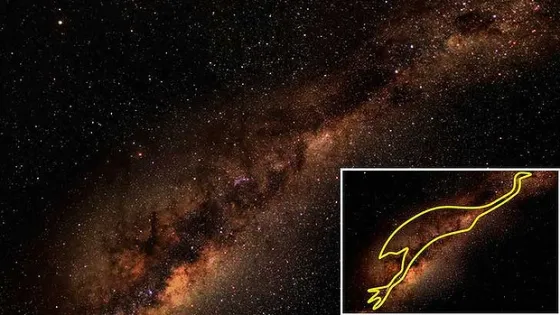
\includegraphics[width=0.7\linewidth]{../screenshot001}
  	\end{center}
  
  \item Other dark constellations: Possum, Caterpillar, Pregnant Woman, Wedge-tailed Eagle
  \item The dark areas are \vocab{molecular clouds}\label{voc:molecular-clouds} --- real, scientifically significant objects and birthplaces of new stars
\end{itemize}


\begin{youdobox}

\question{2}{Explain how a dark constellation differs from a Western constellation.}
\answerbox{1.6cm}

\question{2}{Name the nebula that forms the head of the Emu in the Sky, and the constellation it lies near.}
\answerbox{1.6cm}

\question{3}{Explain what the dark lanes of the Milky Way actually are, and why they are scientifically significant.}
\answerbox{1.6cm}

\question{2}{Describe the ecological information encoded by the position of the Emu in the Sky in autumn.}
\answerbox{1.6cm}

\end{youdobox}

\subsection{The Boorong star catalogue}\label{sub:7.2}

The Boorong people (Wergaia, north-western Victoria) have one of the best-documented Aboriginal astronomical knowledge systems. With the assistance of Elder William Barak, surveyor William Stanbridge documented 47 named celestial objects in 1857:

\begin{itemize}
  \item The Magellanic Clouds (as \textit{Yugarilya})
  \item Open star clusters (Pleiades, Hyades)
  \item Variable stars
  \item A record of the Eta Carinae brightening event of c.1843 (\textit{Collowgulloric War}) --- consistent with European records of the same event
\end{itemize}


\begin{youdobox}

\question{3}{State how many celestial objects were documented in the Boorong catalogue, in what year, and by whom.}
\answerbox{1.6cm}

\question{2}{Name two types of celestial object recorded in the Boorong catalogue.}
\answerbox{1.6cm}

\question{1}{State the Boorong name for the Magellanic Clouds.}
\answerbox{1.6cm}

\question{3}{Explain why the Boorong record of the Eta Carinae brightening is scientifically significant.}
\answerbox{1.6cm}

\end{youdobox}

\subsection{The sky as ecological calendar}\label{sub:7.3}

\begin{countrybox}{Wurundjeri sky knowledge in practice}
On Wurundjeri Country, the rising of the Pleiades (Seven Sisters, \textit{Nurrumbunguttias}) marks the transition between seasons and signals specific ecological activities. The six-season Kulin calendar integrates the position and orientation of stars, the Milky Way, and the Moon to create a precise framework for land management that has been maintained across hundreds of generations.

\medskip
The seasonal position of the Emu in the Sky has been validated by ecologists: when the Emu's body is horizontal above the southern horizon at dusk in autumn, emus are nesting and their eggs are available. This ecological timing is accurate and has been used for at least 65,000 years.
\end{countrybox}

\begin{wedobox}{Your turn --- Evaluating oral knowledge}
A student argues: ``Aboriginal astronomy can't be reliable science because it's not written down.'' Write a three-point rebuttal with specific evidence.

\vspace{6cm}
\end{wedobox}




\begin{youdobox}

\question{2}{Explain what the rising of the Pleiades signals on Wurundjeri Country.}
\answerbox{1.6cm}

\question{3}{Describe two ways the six-season Kulin calendar differs from the European four-season model.}
\answerbox{1.6cm}

\question{3}{Evaluate the claim that Aboriginal astronomy is a science. Use one specific piece of evidence from this lesson.}
\answerbox{1.6cm}

\end{youdobox}


% ABOVE-LEVEL EXTENSION DIVIDER
% Sections 7 and 8 run past the Year 7 level. They sit last so the core
% booklet reads straight through in lesson order; this page marks the
% break for a student working through a printed copy.



\clearpage\markboth{Glossary}{Glossary}\hypertarget{glossary}{}
\subsection*{Glossary}\label{sec:glossary}
{\small Every key word in this booklet and the page it is introduced on.}\par\smallskip
\renewcommand{\arraystretch}{1.3}
\begin{longtable}{|>{\RaggedRight}p{38mm}|p{10mm}|p{\dimexpr\linewidth-48mm-6\tabcolsep-4\arrayrulewidth-1pt\relax}|}
\hline \rule{0pt}{4mm}\headingfont\bfseries Word & \headingfont\bfseries Page & \headingfont\bfseries In my own words \\ \hline \endhead
  Asteroid belt & \pageref{voc:asteroid-belt} & \\ \hline
  AU & \pageref{voc:au} & \\ \hline
  Axial tilt & \pageref{voc:axial-tilt} & \\ \hline
  Climate monitoring & \pageref{voc:climate-monitoring} & \\ \hline
  Comets & \pageref{voc:comets} & \\ \hline
  Crust & \pageref{voc:crust} & \\ \hline
  Dark dust lanes & \pageref{voc:dark-dust-lanes} & \\ \hline
  Dwarf planet & \pageref{voc:dwarf-planet} & \\ \hline
  Dwarf planets & \pageref{voc:dwarf-planets} & \\ \hline
  Elatina Formation & \pageref{voc:elatina-formation} & \\ \hline
  Emergency response & \pageref{voc:emergency-response} & \\ \hline
  Empty space & \pageref{voc:empty-space} & \\ \hline
  Emu in the Sky & \pageref{voc:emu-in-the-sky} & \\ \hline
  GPS & \pageref{voc:gps} & \\ \hline
  Highlands & \pageref{voc:highlands} & \\ \hline
  Inner core & \pageref{voc:inner-core} & \\ \hline
  Kessler syndrome & \pageref{voc:kessler-syndrome} & \\ \hline
  Kuiper Belt & \pageref{voc:kuiper-belt} & \\ \hline
  Lamina & \pageref{voc:lamina} & \\ \hline
  Lunar eclipse & \pageref{voc:lunar-eclipse} & \\ \hline
  Main sequence star & \pageref{voc:main-sequence-star} & \\ \hline
  Mantle & \pageref{voc:mantle} & \\ \hline
  Maria & \pageref{voc:maria} & \\ \hline
  Molecular clouds & \pageref{voc:molecular-clouds} & \\ \hline
  Neap tides & \pageref{voc:neap-tides} & \\ \hline
  Nuclear fusion & \pageref{voc:nuclear-fusion} & \\ \hline
  Oort Cloud & \pageref{voc:oort-cloud} & \\ \hline
  Outer core & \pageref{voc:outer-core} & \\ \hline
  Phases & \pageref{voc:phases} & \\ \hline
  Planar deformation features & \pageref{voc:planar-deformation-features} & \\ \hline
  Planet & \pageref{voc:planet} & \\ \hline
  Precision agriculture & \pageref{voc:precision-agriculture} & \\ \hline
  Reflects sunlight & \pageref{voc:reflects-sunlight} & \\ \hline
  Regolith & \pageref{voc:regolith} & \\ \hline
  Revolves & \pageref{voc:revolves} & \\ \hline
  Rotates & \pageref{voc:rotates} & \\ \hline
  Satellite & \pageref{voc:satellite} & \\ \hline
  Space debris & \pageref{voc:space-debris} & \\ \hline
  Spring tides & \pageref{voc:spring-tides} & \\ \hline
  Tidal braking & \pageref{voc:tidal-braking} & \\ \hline
  Tidal bulge & \pageref{voc:tidal-bulge} & \\ \hline
  Tidal locking & \pageref{voc:tidal-locking} & \\ \hline
  Tidal rhythmite & \pageref{voc:tidal-rhythmite} & \\ \hline
  Weather satellites & \pageref{voc:weather-satellites} & \\ \hline
  West to east & \pageref{voc:west-to-east} & \\ \hline
\end{longtable}
\padtofour
\end{document}
